% Auto-generated by generate_report.py — do not edit manually
% Preamble mirrors oxengthesis.cls so figures match the body text:
% Carlito as main font, Latin Modern Math via unicode-math.
\documentclass[border=6pt]{standalone}
\usepackage{fontspec}
\setmainfont{Carlito}
\usepackage{unicode-math}
\setmathfont{Latin Modern Math}
\usepackage{pgfplots}
\pgfplotsset{compat=1.18}
\usepgfplotslibrary{groupplots}
\usetikzlibrary{patterns,positioning}
\begin{document}
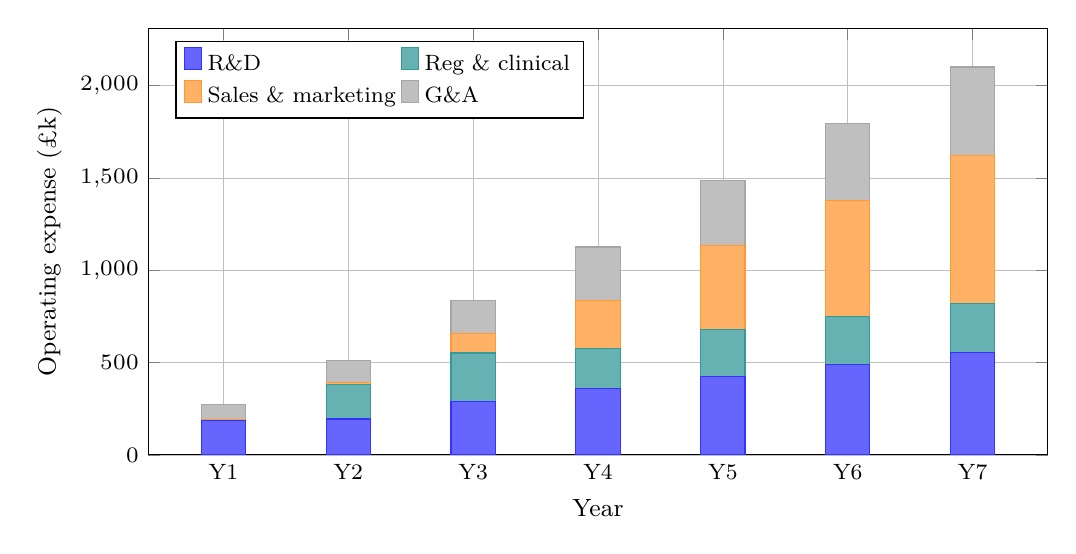
\begin{tikzpicture}
    \begin{axis}[
            width=13cm,
            height=7cm,
            xlabel={Year},
            symbolic x coords={Y1,Y2,Y3,Y4,Y5,Y6,Y7},
            xtick=data,
            grid=major,
            grid style={line width=.1pt, draw=gray!30},
            major grid style={line width=.2pt,draw=gray!50},
            legend style={
                font=\footnotesize,
                at={(0.02,0.98)},
                anchor=north west,
                legend cell align={left},
            },
            tick label style={font=\footnotesize},
            label style={font=\small},
        ylabel={Operating expense (\pounds k)},
        ybar stacked,
        bar width=16pt,
        ymin=0,
        legend pos=north west,
        legend columns=2,
    ]
    \addplot+[ybar,fill=blue!60,draw=blue!80] coordinates {(Y1,184.0) (Y2,194.3) (Y3,286.8) (Y4,357.2) (Y5,422.7) (Y6,488.1) (Y7,553.6)};
    \addplot+[ybar,fill=teal!60,draw=teal!80] coordinates {(Y1,0.0) (Y2,185.5) (Y3,264.9) (Y4,218.6) (Y5,257.3) (Y6,262.3) (Y7,267.3)};
    \addplot+[ybar,fill=orange!60,draw=orange!80] coordinates {(Y1,5.3) (Y2,10.9) (Y3,104.0) (Y4,259.2) (Y5,454.2) (Y6,626.2) (Y7,801.7)};
    \addplot+[ybar,fill=gray!50,draw=gray!70] coordinates {(Y1,81.2) (Y2,121.8) (Y3,178.5) (Y4,291.1) (Y5,354.1) (Y6,417.1) (Y7,478.1)};
    \legend{R\&D, Reg \& clinical, Sales \& marketing, G\&A}
    \end{axis}
\end{tikzpicture}

\end{document}
